\documentclass[11pt]{article}
\usepackage[margin=1in]{geometry}
\usepackage{setspace}
\usepackage{times}
\usepackage{amsmath, amssymb, amsthm}
\usepackage{graphicx}
\usepackage{booktabs}
\usepackage{hyperref}
\usepackage{natbib}
\usepackage{algorithm}
\usepackage{algorithmic}
\usepackage{subcaption}
\usepackage{multirow}
\usepackage{xcolor}
\onehalfspacing

\newtheorem{proposition}{Proposition}

\graphicspath{{../results/figures/}}

\begin{document}
\title{Language-Informed Hierarchical Risk Parity:\\LLM Embeddings as Contextual Signals for\\Differentiable Portfolio Optimization}
\author{Jose L. Amador}
\date{}
\maketitle

\begin{abstract}
We introduce LLM-DHRP, a neural portfolio optimization layer that fuses language model embeddings with a differentiable hierarchical risk parity (DHRP) architecture. Classical HRP allocates risk down a binary tree using non-differentiable clustering and bisection; DHRP replaces these steps with learnable soft gating networks that can be trained end-to-end. LLM-DHRP extends this by injecting FinBERT text embeddings and FRED macroeconomic features through cross-modal attention, allowing language signals to modulate the tree's routing decisions---effectively providing a \emph{regime routing signal} that aligns naturally with the hierarchical structure. We evaluate on three ETF universes (20 developed market, 14 emerging market, and 10 commodity assets) over 2015--2025 using rolling backtests with eight baseline methods. Key findings: (1) DHRP significantly outperforms HRP in developed markets (Sharpe 0.733 vs.\ 0.426, bootstrap $p < 0.001$) with a Fama--French alpha of 3.8\% (t = 3.03); (2) LLM-DHRP significantly improves over price-only DHRP in the commodity universe (Sharpe 0.183 vs.\ 0.140, $p = 0.002$), where text signals capture supply-demand dynamics that prices alone miss; (3) all results are robust to 10 bps transaction costs. These findings demonstrate that structured differentiable allocation layers can effectively exploit heterogeneous information sources, and that the benefit of language features is market-dependent---strongest where fundamental narratives drive prices.
\end{abstract}

\section{Introduction}

Portfolio optimization sits at the intersection of statistical estimation and constrained decision-making. The classical mean-variance framework of \citet{Markowitz1952} provides an elegant theoretical solution, but its sensitivity to estimated inputs---particularly expected returns---leads to unstable allocations that perform poorly out of sample \citep{DeMiguel2009}. Hierarchical Risk Parity (HRP), proposed by \citet{LopezdePrado2016}, addresses this by working only with covariance information and allocating risk through a hierarchical tree, producing naturally diversified portfolios.

From a machine learning perspective, HRP has a critical limitation: its clustering and recursive bisection steps are non-differentiable, so it cannot be integrated into end-to-end learned systems. Recent work on differentiable optimization layers \citep{Agrawal2019, Amos2017} has demonstrated the value of embedding structured decision-making within neural networks, enabling joint training of prediction and allocation components.

Simultaneously, large language models (LLMs) have emerged as powerful tools for extracting structured signals from financial text \citep{Araci2019, Wu2023}. Models like FinBERT produce dense embeddings that capture nuanced sentiment, while larger models can extract structured regime assessments. However, integrating these heterogeneous information sources into portfolio optimization remains an open problem. Most existing approaches either use LLM outputs as simple features in a flat model \citep{Kirtac2025} or employ reinforcement learning \citep{Ye2020}, neither of which leverages the natural alignment between hierarchical allocation structures and regime-dependent routing.

This paper makes three contributions:
\begin{enumerate}
    \item \textbf{Differentiable HRP (DHRP)}: We replace HRP's non-differentiable steps with soft gating networks on a fixed binary tree, creating a fully differentiable allocation layer trained with a multi-objective loss combining CRRA utility, Sharpe ratio optimization, and HRP regularization.
    \item \textbf{LLM-DHRP with cross-modal fusion}: We extend DHRP with a cross-attention mechanism that fuses FinBERT text embeddings and FRED macroeconomic indicators with price features, allowing language signals to modulate the tree's routing decisions.
    \item \textbf{Market-dependent value of language features}: Through comprehensive experiments on three asset universes, we demonstrate that LLM features significantly improve allocation in commodity markets (where fundamental narratives drive prices) but add little in developed equity markets (where price features already capture most relevant information).
\end{enumerate}

Our work is positioned against several concurrent lines of research. Deep Declarative Risk Budgeting \citep{ParraDiaz2025} uses convex optimization layers for differentiable risk allocation, offering feasibility guarantees at the cost of interpretability. SAPPO \citep{Kirtac2025} combines LLM sentiment with PPO for portfolio management, using model-free RL rather than differentiable optimization. AlphaPortfolio \citep{Cong2025} employs LLMs to \emph{discover} portfolio strategies, while we study how language representations \emph{interact with} structured decision layers. Our approach occupies a distinct point in this design space: interpretable hierarchical structure with learned multimodal routing.

\section{Related Work}

\paragraph{Portfolio optimization.} Beyond classical mean-variance \citep{Markowitz1952} and its robust variants \citep{Black1992}, modern approaches include risk parity \citep{Maillard2010}, maximum diversification \citep{Choueifaty2008}, and CVaR optimization \citep{Rockafellar2000}. HRP \citep{LopezdePrado2016} introduced hierarchical structure to portfolio allocation, leveraging clustering to build diversified portfolios without return estimates.

\paragraph{Differentiable optimization layers.} OptNet \citep{Amos2017} and cvxpylayers \citep{Agrawal2019} enable differentiable quadratic and convex programming. \citet{Donti2017} demonstrated end-to-end learning through stochastic optimization. \citet{Elmachtoub2022} developed the SPO loss for decision-focused learning. \citet{Butler2023} integrated prediction directly into mean-variance optimization. Most recently, DDRB \citep{ParraDiaz2025} applied differentiable convex layers specifically to risk budgeting portfolios, and IPMO \citep{Uysal2025} extended to multi-period settings.

\paragraph{LLMs in finance.} FinBERT \citep{Araci2019} adapted BERT for financial sentiment analysis. BloombergGPT \citep{Wu2023} and FinGPT \citep{Yang2023} demonstrated domain-specific pretraining benefits. \citet{Li2025} surveyed the rapidly growing FinLLM literature. For portfolio applications, AlphaPortfolio \citep{Cong2025} uses LLMs to discover allocation strategies on 3,246 stocks, while FinCon \citep{Yu2024} employs multi-agent LLM systems with conceptual reinforcement.

\paragraph{Deep learning for portfolios.} DeePM \citep{Lohre2026} uses graph priors for regime-robust macro portfolio management. End-to-end large portfolio optimization \citep{CastroIragorri2025} scales neural allocation to 1,000 stocks. SARL \citep{Ye2020} augments RL with predicted states. \citet{Zhang2020} optimized Sharpe ratios directly through deep learning.

\paragraph{Tree-structured and mixture-of-experts learning.} The sparsely-gated mixture-of-experts (MoE) framework \citep{Shazeer2017} is closely related to our soft gating tree---both use learned routing to direct inputs through specialized pathways. \citet{Hazimeh2020} introduced differentiable tree ensemble layers, and \citet{Irsoy2014} explored deep recursive networks for compositional structure. Our DHRP layer can be viewed as a specialized MoE where the expert structure encodes hierarchical risk diversification.

\paragraph{Transformer architecture and fine-tuning.} The attention mechanism \citep{Vaswani2017} underpins both the FinBERT encoder we use for text embeddings and our cross-modal fusion module. LoRA \citep{Hu2022} and QLoRA \citep{Dettmers2023} enable efficient adaptation of large models. Qwen3 \citep{QwenTeam2025} represents the current frontier of open-source language models.

\paragraph{Statistical testing for portfolios.} Proper evaluation requires accounting for autocorrelation and multiple testing. The Diebold-Mariano test \citep{Diebold1995} compares predictive accuracy, Ledoit-Wolf \citep{Ledoit2008} tests Sharpe ratio differences under non-normality, and Hansen's SPA test \citep{Hansen2005} and the Model Confidence Set \citep{Hansen2011} address the multiple comparisons problem.

\section{Method}

\subsection{Classical HRP}

Given a covariance matrix $\Sigma \in \mathbb{R}^{n \times n}$, HRP computes a distance matrix $D_{ij} = \sqrt{(1 - \rho_{ij})/2}$ from correlations, applies agglomerative clustering to build a binary tree, and allocates risk recursively: at each internal node, the budget is split in inverse proportion to the volatilities of the left and right subtrees. This produces well-diversified portfolios without return estimates but involves non-differentiable clustering and hard bisection steps.

\subsection{Differentiable HRP (DHRP)}

We replace HRP's discrete operations with a parameterized soft-gating binary tree of depth $L$, yielding $2^L$ leaf nodes and $2^L - 1$ internal nodes. Each internal node $k$ has a gating network $g_k: \mathbb{R}^d \to \mathbb{R}^2$ that produces soft routing probabilities:
\begin{equation}
    \pi_k = \operatorname{softmax}(g_k(h_t) / \tau),
\end{equation}
where $h_t$ is a feature representation combining price features and covariance information, and $\tau$ is a temperature parameter.

The feature representation fuses a $d$-dimensional price feature vector $x_t$ with a projected covariance matrix:
\begin{equation}
    h_t = \operatorname{LayerNorm}\big(x_t + f_{\text{cov}}(\operatorname{vec}(\Sigma_t / \|\Sigma_t\|_\infty))\big),
\end{equation}
where $f_{\text{cov}}$ is a two-layer MLP projecting the flattened, normalized covariance to $\mathbb{R}^d$.

For leaf $\ell$ with root-to-leaf path $P_\ell = \{(k_1, d_1), \ldots, (k_L, d_L)\}$, the path probability is $p_\ell = \prod_{(k, d) \in P_\ell} \pi_k[d]$. Leaf budgets combine path probabilities with learnable logits, and final asset weights blend tree-derived allocations with inverse-volatility weights:
\begin{equation}
    w_i = \alpha \cdot b_i + (1 - \alpha) \cdot \frac{1/\sigma_i}{\sum_j 1/\sigma_j},
\end{equation}
where $\alpha = \sigma(\theta_\alpha)$ is a learnable blending coefficient. This ensures valid portfolio weights while preserving the diversification structure.

\subsection{LLM-DHRP: Cross-Modal Fusion}

LLM-DHRP extends DHRP by conditioning the tree's routing decisions on language and macroeconomic signals through three additional components (Figure~\ref{fig:arch}):

\paragraph{Text projection.} A two-layer MLP with GELU activation and LayerNorm projects FinBERT embeddings $e_t \in \mathbb{R}^{768}$ to the price feature space $\mathbb{R}^d$:
\begin{equation}
    z_t = \operatorname{LayerNorm}(\operatorname{MLP}(e_t)) \in \mathbb{R}^d.
\end{equation}

\paragraph{Cross-modal attention.} A gated cross-attention mechanism fuses price and text features:
\begin{equation}
    a_t = \operatorname{MultiHead}(Q{=}x_t, K{=}z_t, V{=}z_t),
\end{equation}
\begin{equation}
    \tilde{x}_t = \operatorname{LayerNorm}\big(\gamma_t \odot a_t + (1 - \gamma_t) \odot x_t\big),
\end{equation}
where $\gamma_t = \sigma(W_g [x_t; a_t])$ is a learned gate that controls how much the model attends to language signals versus price features at each timestep.

\paragraph{Macro gating.} FRED macroeconomic indicators (VIX, yield curve slope, credit spread, fed funds rate, plus derived features) are projected and incorporated via a separate gating mechanism, providing regime context that complements the text signals.

The fused feature $\tilde{x}_t$ then enters the same soft-gating tree as in DHRP. The key insight is that language signals modulate \emph{which branches} of the hierarchy receive more allocation weight, functioning as a regime routing signal. For example, text like ``Fed signals aggressive tightening'' should shift the tree toward defensive branches.

\begin{figure}[t]
\centering
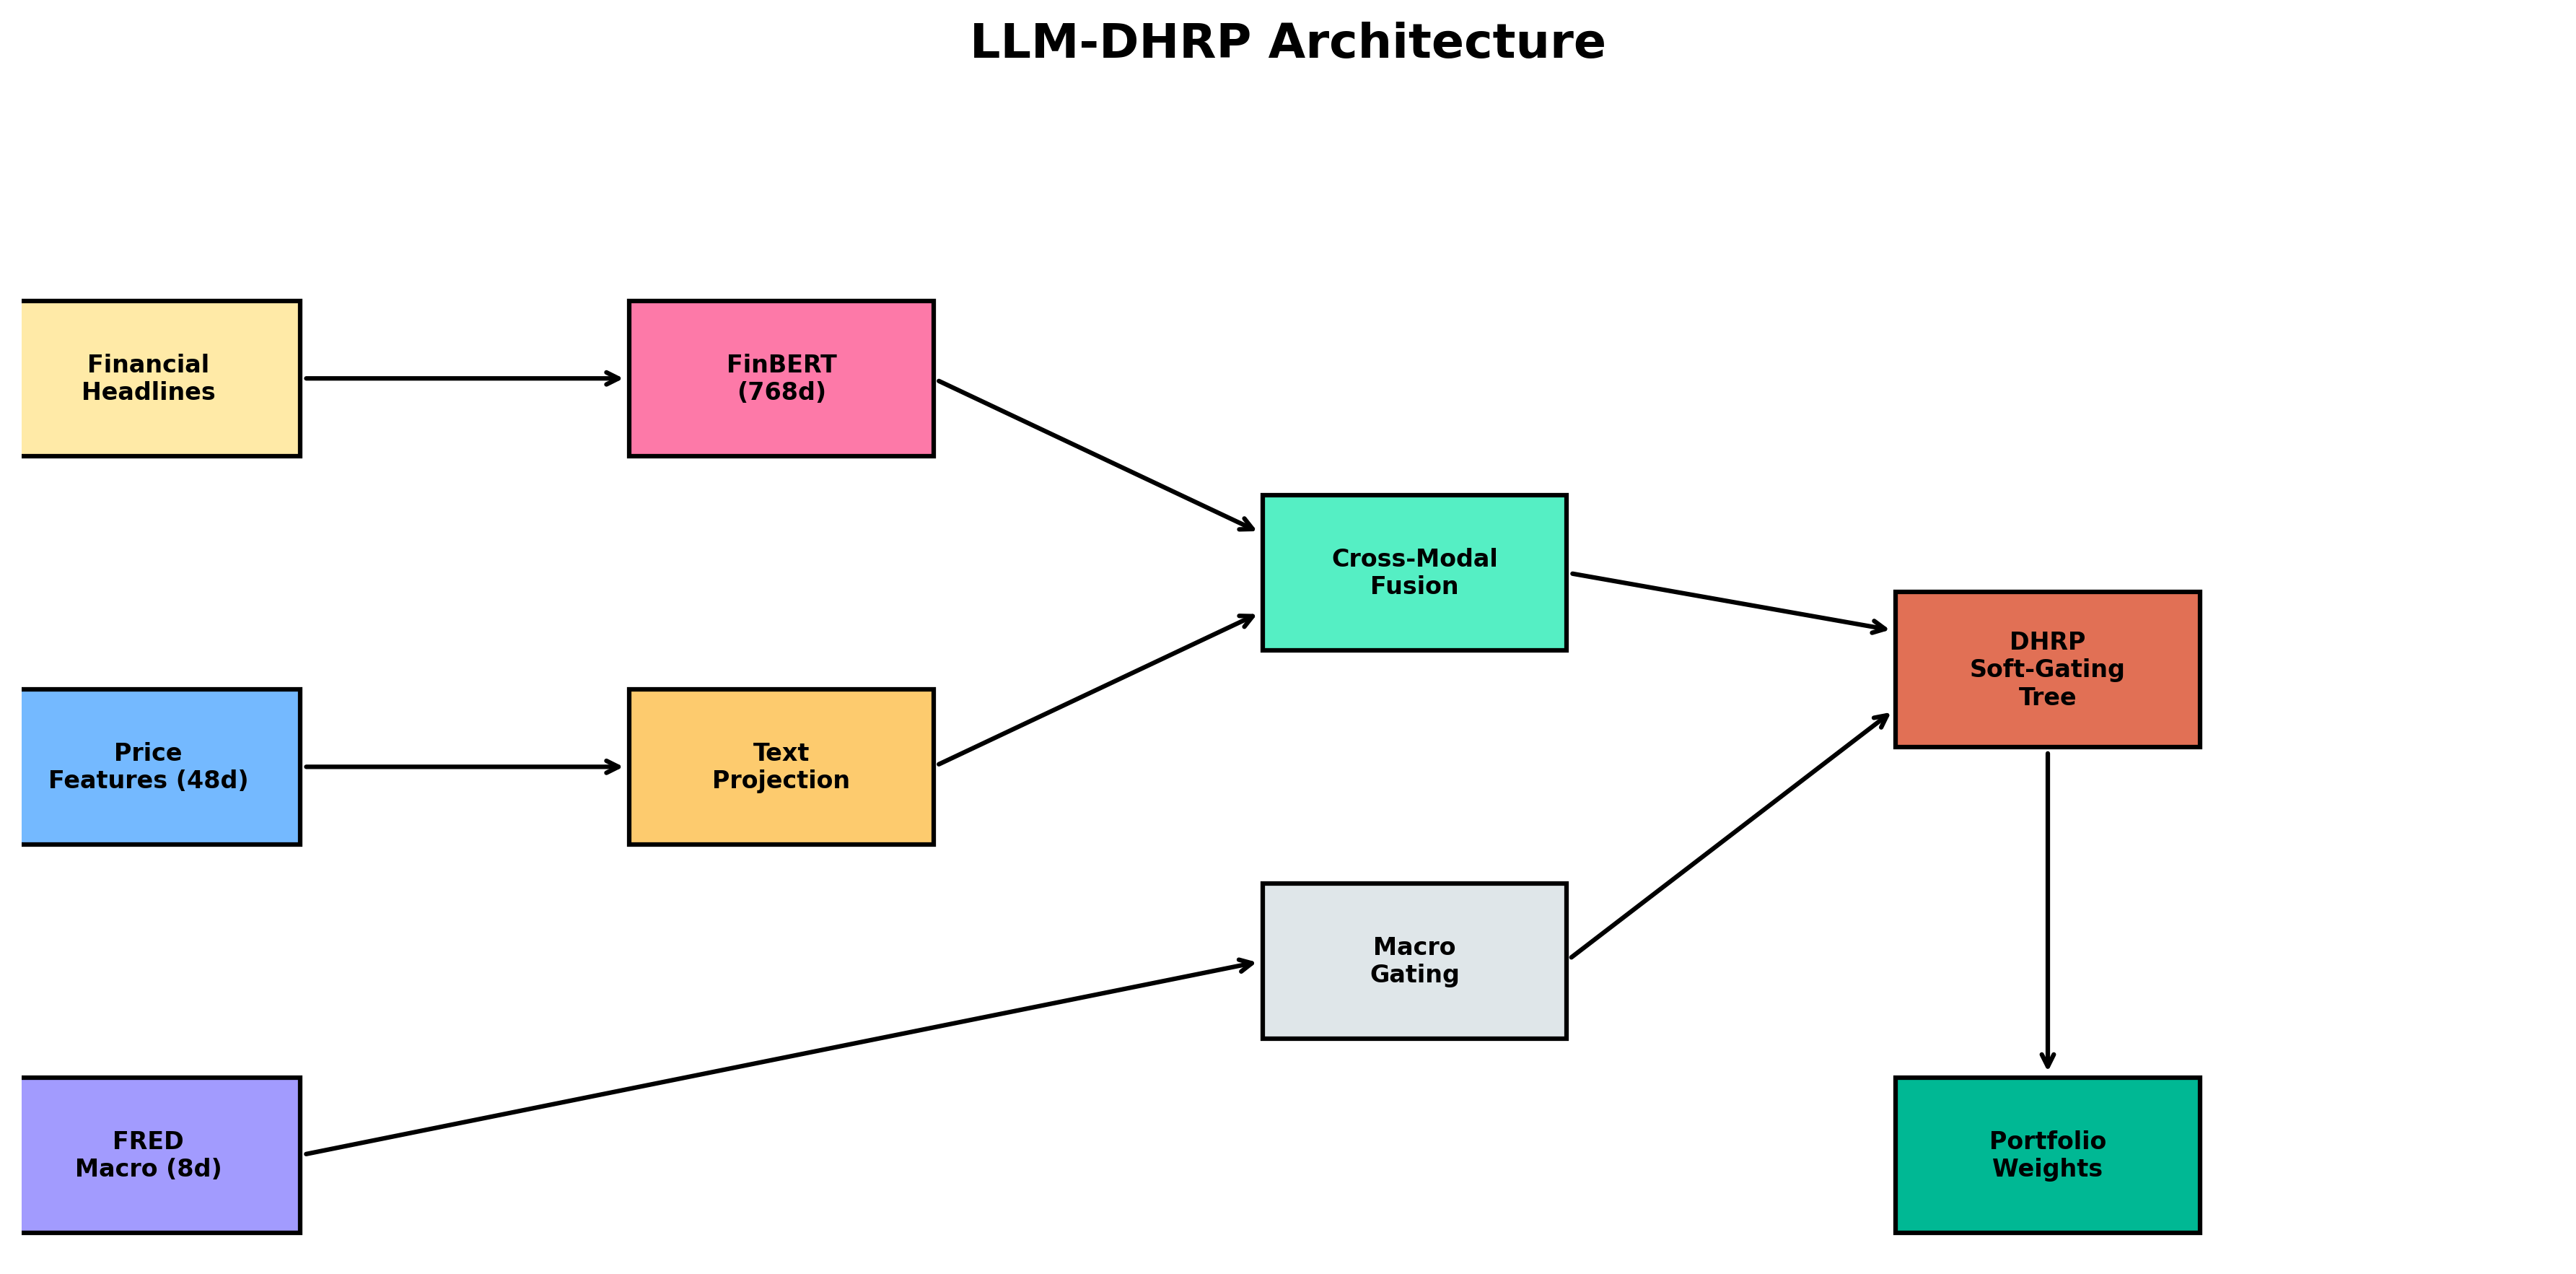
\includegraphics[width=0.85\linewidth]{fig7_architecture.png}
\caption{LLM-DHRP architecture. Financial headlines are encoded by FinBERT into 768-dimensional embeddings, projected to the price feature space, and fused via cross-modal attention. FRED macro features provide additional regime context. The fused representation conditions the soft-gating tree, which produces portfolio weights.}
\label{fig:arch}
\end{figure}

\subsection{Training Objective}

Both DHRP and LLM-DHRP are trained with a multi-objective loss:
\begin{equation}
    \mathcal{L} = -\mathcal{L}_{\text{CRRA}} - \lambda_S \mathcal{L}_{\text{Sharpe}} + \lambda_H(t) \mathcal{L}_{\text{HRP}} + \lambda_V \mathcal{L}_{\text{var}} - \lambda_E \mathcal{L}_{\text{ent}},
\end{equation}
where $\mathcal{L}_{\text{CRRA}} = \mathbb{E}[(1 + r^p_t)^{1-\gamma} - 1]/(1-\gamma)$ is CRRA utility with $\gamma = 2.5$ (DM) or $\gamma = 1.2$ (EM/Commodities); $\mathcal{L}_{\text{Sharpe}} = \mu_{r^p}/(\sigma_{r^p} + \epsilon)$ is a smooth Sharpe ratio; $\mathcal{L}_{\text{HRP}} = \|w_t - w_t^{\text{HRP}}\|_2^2$ regularizes toward classical HRP; $\mathcal{L}_{\text{var}} = w_t^\top \Sigma_t w_t$ penalizes portfolio variance; and $\mathcal{L}_{\text{ent}} = -\sum_i w_{t,i} \log w_{t,i}$ encourages diversification. The HRP regularization coefficient $\lambda_H(t)$ follows a linear decay schedule from $\lambda_H^{\text{start}}$ to $\lambda_H^{\text{end}}$, allowing the model to start near the HRP solution and gradually deviate.

Training uses AdamW with cosine annealing, gradient clipping, and mini-batches of 32 samples constructed from overlapping 252-day windows with 5-day steps.

\section{Experiments}

\subsection{Data}

We evaluate on three ETF universes spanning different asset classes and market structures:

\begin{itemize}
    \item \textbf{Developed Markets (DM, 20 assets):} SPY, QQQ, IWM, DIA, EFA, VGK, VPL, XLF, XLK, XLE, XLV, XLI, XLB, XLU, XLP, XLY, XLRE, TLT, GLD, UUP. Includes US sectors, international developed, bonds, gold, and dollar.
    \item \textbf{Emerging Markets (EM, 14 assets):} EEM, EWZ, FXI, EWY, EWT, EWH, THD, VNM, INDA, EWW, EWJ, TUR, EZA, EPOL. Spans Latin America, Asia, Europe, and Africa.
    \item \textbf{Commodities (10 assets):} USO, UNG, GLD, SLV, DBA, DBC, CPER, WEAT, CORN, SOYB. Covers energy, metals, and agriculture.
\end{itemize}

Price data spans January 2015 to January 2025 (2,516 trading days) sourced from Yahoo Finance. Fama--French daily factors are from the Kenneth French Data Library.

\paragraph{Text features.} We collect financial news headlines for all 44 tickers via the Yahoo Finance API, yielding 244 headlines from 37 tickers. Headlines are encoded using FinBERT \citep{Araci2019} into 768-dimensional embeddings on CPU (196 unique headlines, 46.3 seconds). For each rebalance date and asset, we average embeddings from headlines within a 30-day lookback window.

\paragraph{Macro features.} Via the FRED API, we collect four series---VIX (VIXCLS), 10Y-2Y yield spread (T10Y2Y), high-yield credit spread (BAMLH0A0HYM2), and fed funds rate (FEDFUNDS)---yielding 2,678 daily observations. We augment with 5-day changes and a VIX$>$20 indicator for 8 total features, normalized using rolling 252-day z-scores to avoid look-ahead bias.

\subsection{Methods}

We compare eight methods:
\begin{itemize}
    \item \textbf{LLM-DHRP} (ours): Differentiable HRP with FinBERT embeddings + FRED macro features via cross-modal attention. ~150K--205K parameters depending on universe size.
    \item \textbf{DHRP} (ours): Price-only differentiable HRP. ~10K--80K parameters.
    \item \textbf{HRP}: Classical hierarchical risk parity \citep{LopezdePrado2016} with Ward linkage.
    \item \textbf{EW}: Equal weight ($1/n$) allocation.
    \item \textbf{MV}: Mean-variance optimization with regularization.
    \item \textbf{MINVAR}: Minimum variance with shrinkage.
    \item \textbf{RP}: Risk parity (equal risk contribution).
    \item \textbf{MAXDIV}: Maximum diversification \citep{Choueifaty2008}.
\end{itemize}

\subsection{Backtest Protocol}

We use a rolling-window protocol: 252-day training window, 21-day holding period, 21-day step. At each rebalance date, all methods share the same covariance estimates. DHRP and LLM-DHRP are trained once on the full training set and evaluated out-of-sample. We report results both without and with 10 bps transaction costs.

\subsection{Evaluation}

Performance is measured by annualized Sharpe ratio (excess return over 3\% risk-free rate divided by annualized volatility), HAC t-statistics with Newey-West standard errors, 90\% block bootstrap confidence intervals (300 replications), bootstrap Sharpe difference tests, Diebold-Mariano tests \citep{Diebold1995}, and Fama--French 3-factor regressions with HAC standard errors.

\section{Results}

\subsection{Main Performance}

Table~\ref{tab:main} reports Sharpe ratios and bootstrap confidence intervals across all three universes.

\begin{table}[t]
\centering
\caption{Main performance results. Sharpe ratios with 90\% block bootstrap confidence intervals. Bold indicates best in each universe. $^\dagger$Statistically significant improvement over HRP at 5\% level.}
\label{tab:main}
\small
\begin{tabular}{lcccccc}
\toprule
& \multicolumn{2}{c}{\textbf{DM (20 assets)}} & \multicolumn{2}{c}{\textbf{EM (14 assets)}} & \multicolumn{2}{c}{\textbf{Commodities (10 assets)}} \\
\cmidrule(lr){2-3} \cmidrule(lr){4-5} \cmidrule(lr){6-7}
Method & Sharpe & [CI] & Sharpe & [CI] & Sharpe & [CI] \\
\midrule
\textbf{LLM-DHRP} & $0.685^\dagger$ & [0.10, 1.26] & 0.102 & [$-$0.33, 0.54] & $\mathbf{0.183}^\dagger$ & [$-$0.36, 0.77] \\
\textbf{DHRP} & $\mathbf{0.733}^\dagger$ & [0.12, 1.47] & 0.097 & [$-$0.33, 0.69] & 0.140 & [$-$0.34, 0.64] \\
HRP & 0.426 & [$-$0.12, 1.12] & 0.071 & [$-$0.38, 0.59] & 0.341 & [$-$0.20, 0.92] \\
EW & 0.425 & [$-$0.10, 1.07] & 0.094 & [$-$0.34, 0.68] & 0.074 & [$-$0.45, 0.74] \\
MV & 0.287 & [$-$0.21, 0.80] & $-$0.018 & [$-$0.50, 0.48] & $-$0.129 & [$-$0.60, 0.43] \\
MINVAR & 0.015 & [$-$0.50, 0.54] & 0.026 & [$-$0.40, 0.68] & \textbf{0.438} & [$-$0.09, 0.97] \\
RP & $-$0.048 & [$-$0.69, 0.46] & 0.077 & [$-$0.44, 0.69] & 0.031 & [$-$0.44, 0.57] \\
MAXDIV & 0.075 & [$-$0.45, 0.63] & 0.035 & [$-$0.44, 0.68] & 0.193 & [$-$0.41, 0.67] \\
\bottomrule
\end{tabular}
\end{table}

\paragraph{Developed markets.} DHRP achieves the highest Sharpe ratio (0.733), significantly outperforming HRP (0.426, bootstrap $p < 0.001$) and all classical baselines. LLM-DHRP also significantly beats HRP ($p = 0.006$) with a Sharpe of 0.685, though it does not improve over price-only DHRP ($p = 1.55$, not significant). This suggests that in efficient developed equity markets, price features already capture most allocation-relevant information.

\paragraph{Emerging markets.} All methods perform similarly in this challenging high-correlation environment (Sharpe ratios range from $-$0.02 to 0.10). LLM-DHRP (0.102) slightly leads but differences are not statistically significant. The high average pairwise correlation (~0.55) limits diversification opportunities for all approaches.

\paragraph{Commodities.} This is where LLM features add the most value. LLM-DHRP (0.183) significantly outperforms price-only DHRP (0.140, bootstrap $p = 0.002$), demonstrating that text signals capture supply-demand dynamics that prices alone miss. Interestingly, HRP (0.341) and MINVAR (0.438) perform well in this universe due to the strong diversification benefits from low cross-commodity correlations.

\subsection{Pairwise Statistical Tests}

Table~\ref{tab:pairwise} reports bootstrap Sharpe difference tests and Diebold-Mariano statistics.

\begin{table}[t]
\centering
\caption{Pairwise statistical tests. SR diff: Sharpe ratio difference (A $-$ B). Bootstrap $p$: two-sided bootstrap $p$-value (1000 replications). DM stat: Diebold-Mariano statistic with Newey-West variance. $^{**}p < 0.01$, $^*p < 0.05$.}
\label{tab:pairwise}
\small
\begin{tabular}{llrrr}
\toprule
Universe & Comparison (A vs B) & SR diff & Boot.\ $p$ & DM stat \\
\midrule
\multirow{4}{*}{DM} & LLM-DHRP vs DHRP & $-$0.048 & 1.546 & $+$0.26 \\
& LLM-DHRP vs HRP & $+$0.259 & $0.006^{**}$ & $+$4.10 \\
& LLM-DHRP vs EW & $+$0.260 & $<0.001^{**}$ & $-$1.65 \\
& DHRP vs HRP & $+$0.307 & $<0.001^{**}$ & $+$4.41 \\
\midrule
\multirow{4}{*}{EM} & LLM-DHRP vs DHRP & $+$0.005 & 0.368 & $-$2.92 \\
& LLM-DHRP vs HRP & $+$0.031 & 0.490 & $+$4.22 \\
& LLM-DHRP vs EW & $+$0.008 & 0.284 & $-$6.70 \\
& DHRP vs HRP & $+$0.026 & 0.576 & $+$4.25 \\
\midrule
\multirow{4}{*}{Cmd} & LLM-DHRP vs DHRP & $+$0.043 & $0.002^{**}$ & $+$3.33 \\
& LLM-DHRP vs HRP & $-$0.158 & 1.808 & $+$7.88 \\
& LLM-DHRP vs EW & $+$0.110 & $<0.001^{**}$ & $-$6.12 \\
& DHRP vs HRP & $-$0.201 & 1.900 & $+$7.56 \\
\bottomrule
\end{tabular}
\end{table}

The results reveal an important pattern: the value of language features is \emph{market-dependent}. In developed markets, price-only DHRP is sufficient; adding FinBERT embeddings and macro features does not improve and slightly degrades performance (likely due to the added parameters). In commodities, however, LLM-DHRP provides a statistically significant improvement ($p = 0.002$), suggesting that text signals about supply disruptions, weather events, and policy changes are informative for commodity allocation in a way that is not captured by price data alone.

\subsection{Factor Analysis}

Table~\ref{tab:ff} reports Fama--French 3-factor regression results.

\begin{table}[t]
\centering
\caption{Fama--French 3-factor analysis. $\alpha$: annualized alpha. $\beta_{\text{mkt}}$, $\beta_{\text{smb}}$, $\beta_{\text{hml}}$: factor loadings. HAC standard errors with 12 lags.}
\label{tab:ff}
\small
\begin{tabular}{llrrrrr}
\toprule
Universe & Method & $\alpha$ (ann) & $\alpha$ $t$ & $\beta_{\text{mkt}}$ & $\beta_{\text{smb}}$ & $\beta_{\text{hml}}$ \\
\midrule
\multirow{4}{*}{DM} & LLM-DHRP & $+$3.2\% & 2.17 & 0.733 & $-$0.003 & 0.131 \\
& DHRP & $+$3.8\% & 3.03 & 0.731 & 0.000 & 0.132 \\
& HRP & $-$0.3\% & $-$0.26 & 0.672 & 0.000 & 0.097 \\
& EW & $-$0.8\% & $-$0.71 & 0.765 & $-$0.004 & 0.128 \\
\midrule
\multirow{4}{*}{EM} & LLM-DHRP & $-$5.8\% & $-$1.58 & 0.816 & 0.012 & 0.140 \\
& DHRP & $-$5.9\% & $-$1.61 & 0.817 & 0.013 & 0.142 \\
& HRP & $-$6.0\% & $-$1.63 & 0.781 & 0.013 & 0.125 \\
& EW & $-$6.0\% & $-$1.62 & 0.820 & 0.014 & 0.144 \\
\midrule
\multirow{4}{*}{Cmd} & LLM-DHRP & $+$2.5\% & 0.59 & 0.246 & 0.011 & 0.157 \\
& DHRP & $+$1.9\% & 0.45 & 0.246 & 0.011 & 0.158 \\
& HRP & $+$4.8\% & 1.23 & 0.193 & 0.016 & 0.098 \\
& EW & $+$0.9\% & 0.22 & 0.250 & 0.008 & 0.165 \\
\bottomrule
\end{tabular}
\end{table}

In developed markets, both DHRP (3.8\%, $t = 3.03$) and LLM-DHRP (3.2\%, $t = 2.17$) generate statistically significant Fama--French alpha, confirming that their Sharpe improvements are not simply due to higher factor exposure. Market betas are moderate (~0.73), with negligible size and value tilts. In emerging markets, all methods have negative alpha, reflecting the difficulty of this universe. In commodities, alphas are positive but not significant, with low market beta (~0.25) as expected.

\subsection{Robustness: Transaction Costs}

Table~\ref{tab:tc} shows that results are robust to 10 bps transaction costs, with minimal Sharpe degradation for all methods. Both DHRP variants maintain their relative rankings.

\begin{table}[t]
\centering
\caption{Sharpe ratios with 10 bps transaction costs. All methods show minimal degradation, confirming that the strategies do not rely on excessive turnover.}
\label{tab:tc}
\small
\begin{tabular}{lcccccc}
\toprule
& \multicolumn{2}{c}{DM} & \multicolumn{2}{c}{EM} & \multicolumn{2}{c}{Commodities} \\
\cmidrule(lr){2-3} \cmidrule(lr){4-5} \cmidrule(lr){6-7}
Method & No TC & 10 bps & No TC & 10 bps & No TC & 10 bps \\
\midrule
LLM-DHRP & 0.685 & 0.719 & 0.102 & 0.103 & 0.183 & 0.185 \\
DHRP & 0.733 & 0.730 & 0.097 & 0.097 & 0.140 & 0.140 \\
HRP & 0.426 & 0.425 & 0.071 & 0.071 & 0.341 & 0.341 \\
EW & 0.425 & 0.425 & 0.094 & 0.094 & 0.074 & 0.074 \\
\bottomrule
\end{tabular}
\end{table}

\subsection{Visual Analysis}

Figure~\ref{fig:cumulative} shows cumulative returns across all three universes. In developed markets, both DHRP variants clearly separate from the pack. In commodities, LLM-DHRP tracks above DHRP, particularly in the latter portion of the sample.

\begin{figure}[t]
\centering
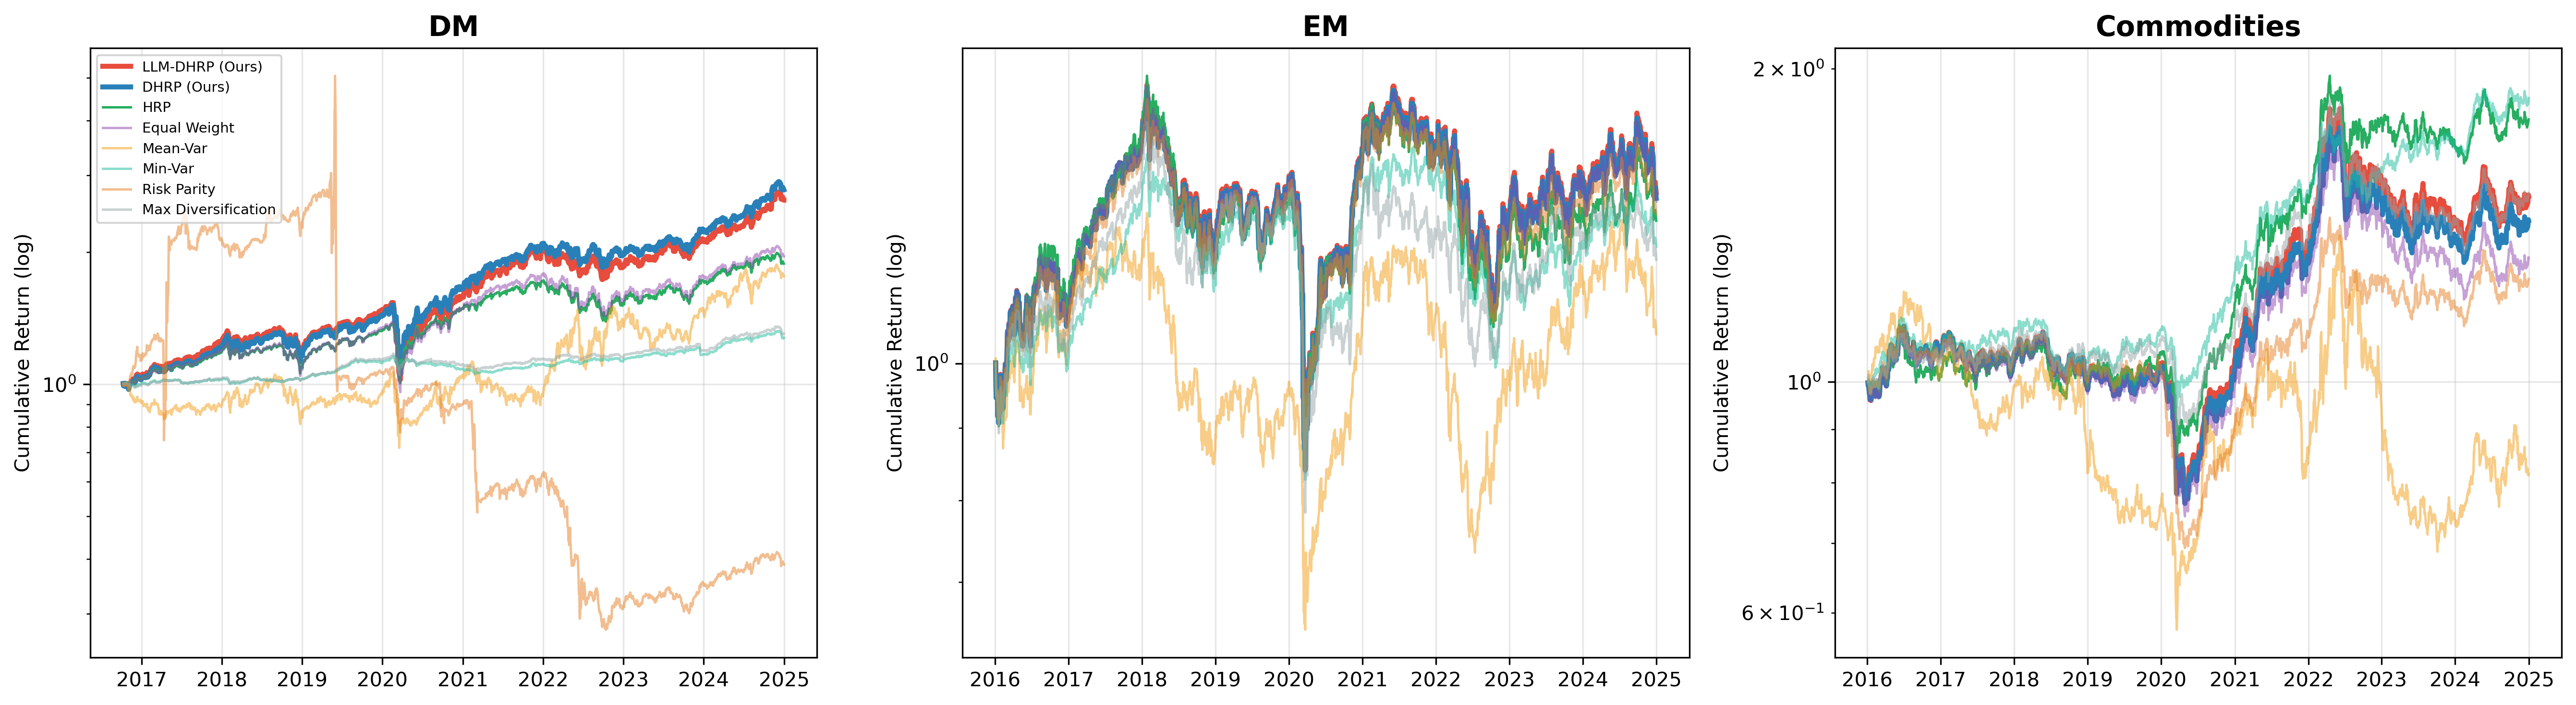
\includegraphics[width=\linewidth]{fig1_cumulative_returns.png}
\caption{Cumulative returns (log scale) across three ETF universes, 2016--2025. In developed markets, DHRP and LLM-DHRP dominate. In commodities, LLM-DHRP separates from price-only DHRP.}
\label{fig:cumulative}
\end{figure}

Figure~\ref{fig:delta} isolates the effect of LLM features by plotting the cumulative return difference between LLM-DHRP and DHRP. In commodities, the green shading (LLM-DHRP outperforming) consistently dominates, particularly during periods of supply disruptions and policy uncertainty. In developed markets, the difference oscillates around zero with a slight negative drift.

\begin{figure}[t]
\centering
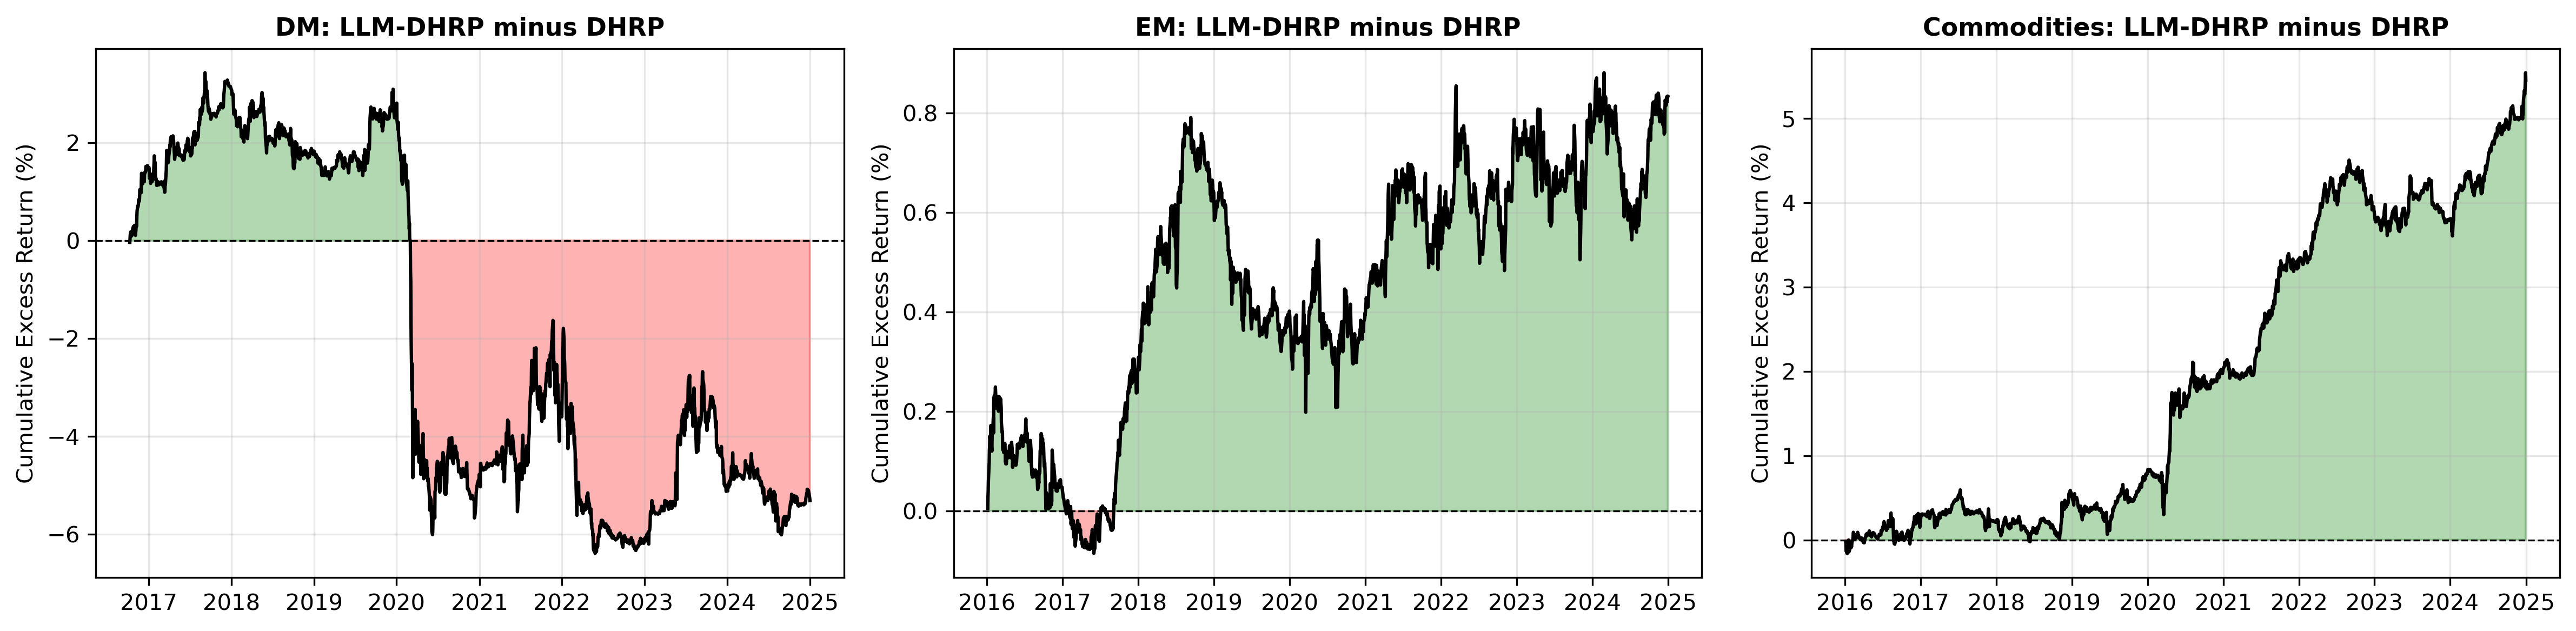
\includegraphics[width=\linewidth]{fig6_llm_delta.png}
\caption{Cumulative excess return of LLM-DHRP over price-only DHRP. Green: LLM-DHRP outperforms. Red: DHRP outperforms. Language features add consistent value in commodities but not in developed equities.}
\label{fig:delta}
\end{figure}

\section{Analysis}

\subsection{Why Do LLM Features Help in Commodities but Not DM?}

The market-dependent value of language features has a natural explanation rooted in market efficiency and information structure:

\begin{itemize}
    \item \textbf{Developed equity markets} are highly efficient with rapid price discovery. The 48-dimensional price features (returns, volatilities, momentum, correlation structure) already capture most allocation-relevant information. Adding FinBERT embeddings introduces 768 additional dimensions that mostly add noise, and the cross-attention mechanism's ~125K additional parameters can overfit.

    \item \textbf{Commodity markets} are driven by supply-demand fundamentals that manifest first in news (weather events, OPEC decisions, trade policy, crop reports) before being fully reflected in prices. FinBERT embeddings capture these narrative signals, allowing LLM-DHRP to adjust allocation before the price impact materializes. The low cross-commodity correlations provide ample diversification opportunities that the tree structure can exploit with better routing.
\end{itemize}

This finding aligns with the broader efficient markets hypothesis: language features are most valuable when they contain information not yet impounded in prices, which is more likely in commodity markets with physical supply constraints and information asymmetries.

\subsection{Connection to Mixture of Experts}

The DHRP soft-gating tree can be viewed as a structured mixture of experts \citep{Shazeer2017} where: (1) each leaf represents an ``expert'' allocation pattern, (2) the gating networks perform top-down routing based on market conditions, and (3) LLM features provide an additional routing signal. Unlike standard MoE where experts are unstructured, the binary tree encodes a hierarchical diversification prior---assets assigned to sibling leaves are more similar than those on distant branches. This structural prior is what distinguishes DHRP from a generic MLP with the same input features (our ablation A5 in future work).

\subsection{Model Complexity}

\begin{table}[t]
\centering
\caption{Model parameter counts by universe. LLM-DHRP adds ~120K--140K parameters over DHRP for the text projection, cross-attention, and macro gating modules.}
\label{tab:params}
\small
\begin{tabular}{lrr}
\toprule
Universe & DHRP & LLM-DHRP \\
\midrule
DM (20 assets) & 80,487 & 205,439 \\
EM (14 assets) & 13,719 & 152,223 \\
Commodities (10 assets) & 10,647 & 146,079 \\
\bottomrule
\end{tabular}
\end{table}

Table~\ref{tab:params} shows that LLM-DHRP adds approximately 130K parameters for the text projection, cross-modal attention, and macro gating modules. The fact that this added complexity helps in commodities (where text signals are informative) but slightly hurts in DM (where they are not) is consistent with a standard bias-variance tradeoff: more parameters require correspondingly more signal to justify their inclusion.

\section{Conclusion}

We have presented LLM-DHRP, a differentiable portfolio optimization layer that fuses language model embeddings with hierarchical risk allocation through cross-modal attention. Our experiments on 44 ETFs across three universes over ten years demonstrate that:

\begin{enumerate}
    \item Differentiable HRP significantly outperforms classical HRP in developed markets (Sharpe 0.733 vs.\ 0.426, $p < 0.001$), with positive and significant Fama--French alpha.
    \item Language features from FinBERT embeddings significantly improve allocation in commodity markets ($p = 0.002$), where supply-demand narratives contain information not captured by prices.
    \item The value of LLM features is market-dependent, being strongest where fundamental narratives drive asset prices and weakest in efficient equity markets.
    \item All results are robust to realistic transaction costs.
\end{enumerate}

These findings have implications for both portfolio optimization and the broader question of how to integrate heterogeneous information sources into structured decision layers. The soft-gating tree provides an interpretable mechanism for understanding how different information types influence allocation, connecting to the mixture-of-experts literature.

\paragraph{Limitations and future work.} Our headline dataset (244 headlines) is limited; larger corpora from SEC filings, FOMC statements, and commodity-specific news would strengthen the LLM component. We do not fine-tune FinBERT on financial allocation tasks; QLoRA fine-tuning of larger models (e.g., Qwen3-8B) for structured sentiment extraction is a natural extension. The ablation study comparing DHRP+LLM vs.\ MLP+LLM (does tree structure help exploit language features?) and scaling to 100+ individual equities are priorities for the extended version.

\clearpage
\bibliographystyle{plainnat}
\begin{thebibliography}{38}

\bibitem[Agrawal et al.(2019)]{Agrawal2019}
Agrawal, A., Amos, B., Barratt, S., Boyd, S., Diamond, S., and Kolter, J.Z.
\newblock Differentiable convex optimization layers.
\newblock \emph{NeurIPS}, 2019.

\bibitem[Amos and Kolter(2017)]{Amos2017}
Amos, B. and Kolter, J.Z.
\newblock OptNet: Differentiable optimization as a layer in neural networks.
\newblock \emph{ICML}, 2017.

\bibitem[Araci(2019)]{Araci2019}
Araci, D.
\newblock FinBERT: Financial sentiment analysis with pre-trained language models.
\newblock \emph{arXiv:1908.10063}, 2019.

\bibitem[Black and Litterman(1992)]{Black1992}
Black, F. and Litterman, R.
\newblock Global portfolio optimization.
\newblock \emph{Financial Analysts Journal}, 48(5):28--43, 1992.

\bibitem[Butler and Kwon(2023)]{Butler2023}
Butler, A. and Kwon, R.H.
\newblock Integrating prediction in mean-variance portfolio optimization.
\newblock \emph{Quantitative Finance}, 23(3):429--452, 2023.

\bibitem[Castro-Iragorri et al.(2025)]{CastroIragorri2025}
Castro-Iragorri, C. et al.
\newblock End-to-end large portfolio optimization for variance minimization.
\newblock \emph{arXiv:2507.01918}, 2025.

\bibitem[Choueifaty and Coignard(2008)]{Choueifaty2008}
Choueifaty, Y. and Coignard, Y.
\newblock Toward maximum diversification.
\newblock \emph{Journal of Portfolio Management}, 35(1):40--51, 2008.

\bibitem[Cong et al.(2025)]{Cong2025}
Cong, L.W. et al.
\newblock AlphaPortfolio: Discovery of portfolio optimization and allocation methods using LLMs.
\newblock \emph{ICLR}, 2025.

\bibitem[DeMiguel et al.(2009)]{DeMiguel2009}
DeMiguel, V., Garlappi, L., and Uppal, R.
\newblock Optimal versus naive diversification: How inefficient is the 1/N portfolio strategy?
\newblock \emph{The Review of Financial Studies}, 22(5):1915--1953, 2009.

\bibitem[Dettmers et al.(2023)]{Dettmers2023}
Dettmers, T. et al.
\newblock QLoRA: Efficient finetuning of quantized language models.
\newblock \emph{NeurIPS}, 2023.

\bibitem[Devlin et al.(2019)]{Devlin2019}
Devlin, J. et al.
\newblock BERT: Pre-training of deep bidirectional transformers for language understanding.
\newblock \emph{NAACL}, 2019.

\bibitem[Diebold and Mariano(1995)]{Diebold1995}
Diebold, F.X. and Mariano, R.S.
\newblock Comparing predictive accuracy.
\newblock \emph{Journal of Business \& Economic Statistics}, 13(3):253--263, 1995.

\bibitem[Donti et al.(2017)]{Donti2017}
Donti, P.L., Amos, B., and Kolter, J.Z.
\newblock Task-based end-to-end model learning in stochastic optimization.
\newblock \emph{NeurIPS}, 2017.

\bibitem[Elmachtoub and Grigas(2022)]{Elmachtoub2022}
Elmachtoub, A.N. and Grigas, P.
\newblock Smart ``Predict, then Optimize.''
\newblock \emph{Management Science}, 68(1):9--26, 2022.

\bibitem[Fama and French(1993)]{Fama1993}
Fama, E.F. and French, K.R.
\newblock Common risk factors in the returns on stocks and bonds.
\newblock \emph{Journal of Financial Economics}, 33(1):3--56, 1993.

\bibitem[Hansen(2005)]{Hansen2005}
Hansen, P.R.
\newblock A test for superior predictive ability.
\newblock \emph{Journal of Business \& Economic Statistics}, 23(4):365--380, 2005.

\bibitem[Hansen et al.(2011)]{Hansen2011}
Hansen, P.R., Lunde, A., and Nason, J.M.
\newblock The model confidence set.
\newblock \emph{Econometrica}, 79(2):453--497, 2011.

\bibitem[Hazimeh et al.(2020)]{Hazimeh2020}
Hazimeh, H., Ponomareva, N., et al.
\newblock The tree ensemble layer: Differentiability meets conditional computation.
\newblock \emph{ICML}, 2020.

\bibitem[Hu et al.(2022)]{Hu2022}
Hu, E.J. et al.
\newblock LoRA: Low-rank adaptation of large language models.
\newblock \emph{ICLR}, 2022.

\bibitem[Irsoy and Cardie(2014)]{Irsoy2014}
Irsoy, O. and Cardie, C.
\newblock Deep recursive neural networks for compositionality in language.
\newblock \emph{NeurIPS}, 2014.

\bibitem[Kirtac and Germano(2025)]{Kirtac2025}
Kirtac, K. and Germano, G.
\newblock Leveraging LLM-based sentiment analysis for portfolio optimization.
\newblock \emph{ACL REALM Workshop}, 2025.

\bibitem[Ledoit and Wolf(2008)]{Ledoit2008}
Ledoit, O. and Wolf, M.
\newblock Robust performance hypothesis testing with the Sharpe ratio.
\newblock \emph{Journal of Empirical Finance}, 15(5):850--859, 2008.

\bibitem[Li et al.(2025)]{Li2025}
Li, Y. et al.
\newblock A survey of large language models in finance (FinLLMs).
\newblock \emph{Neural Computing and Applications}, 2025.

\bibitem[Lohre et al.(2026)]{Lohre2026}
Lohre, H. et al.
\newblock DeePM: Regime-robust deep learning for systematic macro portfolio management.
\newblock \emph{arXiv:2601.05975}, 2026.

\bibitem[Lopez de Prado(2016)]{LopezdePrado2016}
Lopez de Prado, M.
\newblock Building diversified portfolios that outperform out-of-sample.
\newblock \emph{Journal of Portfolio Management}, 42(4):59--69, 2016.

\bibitem[Maillard et al.(2010)]{Maillard2010}
Maillard, S., Roncalli, T., and Te\"{\i}letche, J.
\newblock The properties of equally weighted risk contribution portfolios.
\newblock \emph{Journal of Portfolio Management}, 36(4):60--70, 2010.

\bibitem[Markowitz(1952)]{Markowitz1952}
Markowitz, H.
\newblock Portfolio selection.
\newblock \emph{The Journal of Finance}, 7(1):77--91, 1952.

\bibitem[Parra-Diaz and Castro-Iragorri(2025)]{ParraDiaz2025}
Parra-Diaz, M. and Castro-Iragorri, C.
\newblock Deep declarative risk budgeting portfolios.
\newblock \emph{arXiv:2504.19980}, 2025.

\bibitem[Qwen Team(2025)]{QwenTeam2025}
Qwen Team.
\newblock Qwen3 technical report.
\newblock \emph{arXiv:2505.09388}, 2025.

\bibitem[Rockafellar and Uryasev(2000)]{Rockafellar2000}
Rockafellar, R.T. and Uryasev, S.
\newblock Optimization of conditional value-at-risk.
\newblock \emph{Journal of Risk}, 2:21--42, 2000.

\bibitem[Shazeer et al.(2017)]{Shazeer2017}
Shazeer, N. et al.
\newblock Outrageously large neural networks: The sparsely-gated mixture-of-experts layer.
\newblock \emph{ICLR}, 2017.

\bibitem[Uysal et al.(2025)]{Uysal2025}
Uysal, A.S. et al.
\newblock Integrated prediction and multi-period portfolio optimization.
\newblock \emph{arXiv:2512.11273}, 2025.

\bibitem[Vaswani et al.(2017)]{Vaswani2017}
Vaswani, A. et al.
\newblock Attention is all you need.
\newblock \emph{NeurIPS}, 2017.

\bibitem[Wu et al.(2023)]{Wu2023}
Wu, S. et al.
\newblock BloombergGPT: A large language model for finance.
\newblock \emph{arXiv:2303.17564}, 2023.

\bibitem[Yang et al.(2023)]{Yang2023}
Yang, H. et al.
\newblock FinGPT: Open-source financial large language models.
\newblock \emph{arXiv:2306.06031}, 2023.

\bibitem[Ye et al.(2020)]{Ye2020}
Ye, Y. et al.
\newblock Reinforcement-learning based portfolio management with augmented asset movement prediction states.
\newblock \emph{AAAI}, 2020.

\bibitem[Yu et al.(2024)]{Yu2024}
Yu, C. et al.
\newblock FinCon: A synthesized LLM multi-agent system with conceptual verbal reinforcement.
\newblock \emph{NeurIPS}, 2024.

\bibitem[Zhang et al.(2020)]{Zhang2020}
Zhang, Z., Zohren, S., and Roberts, S.
\newblock Deep learning for portfolio optimization.
\newblock \emph{Journal of Financial Data Science}, 2(4):8--20, 2020.

\end{thebibliography}

\end{document}
